\chapter{Demonstration slides}

\begin{figure}
    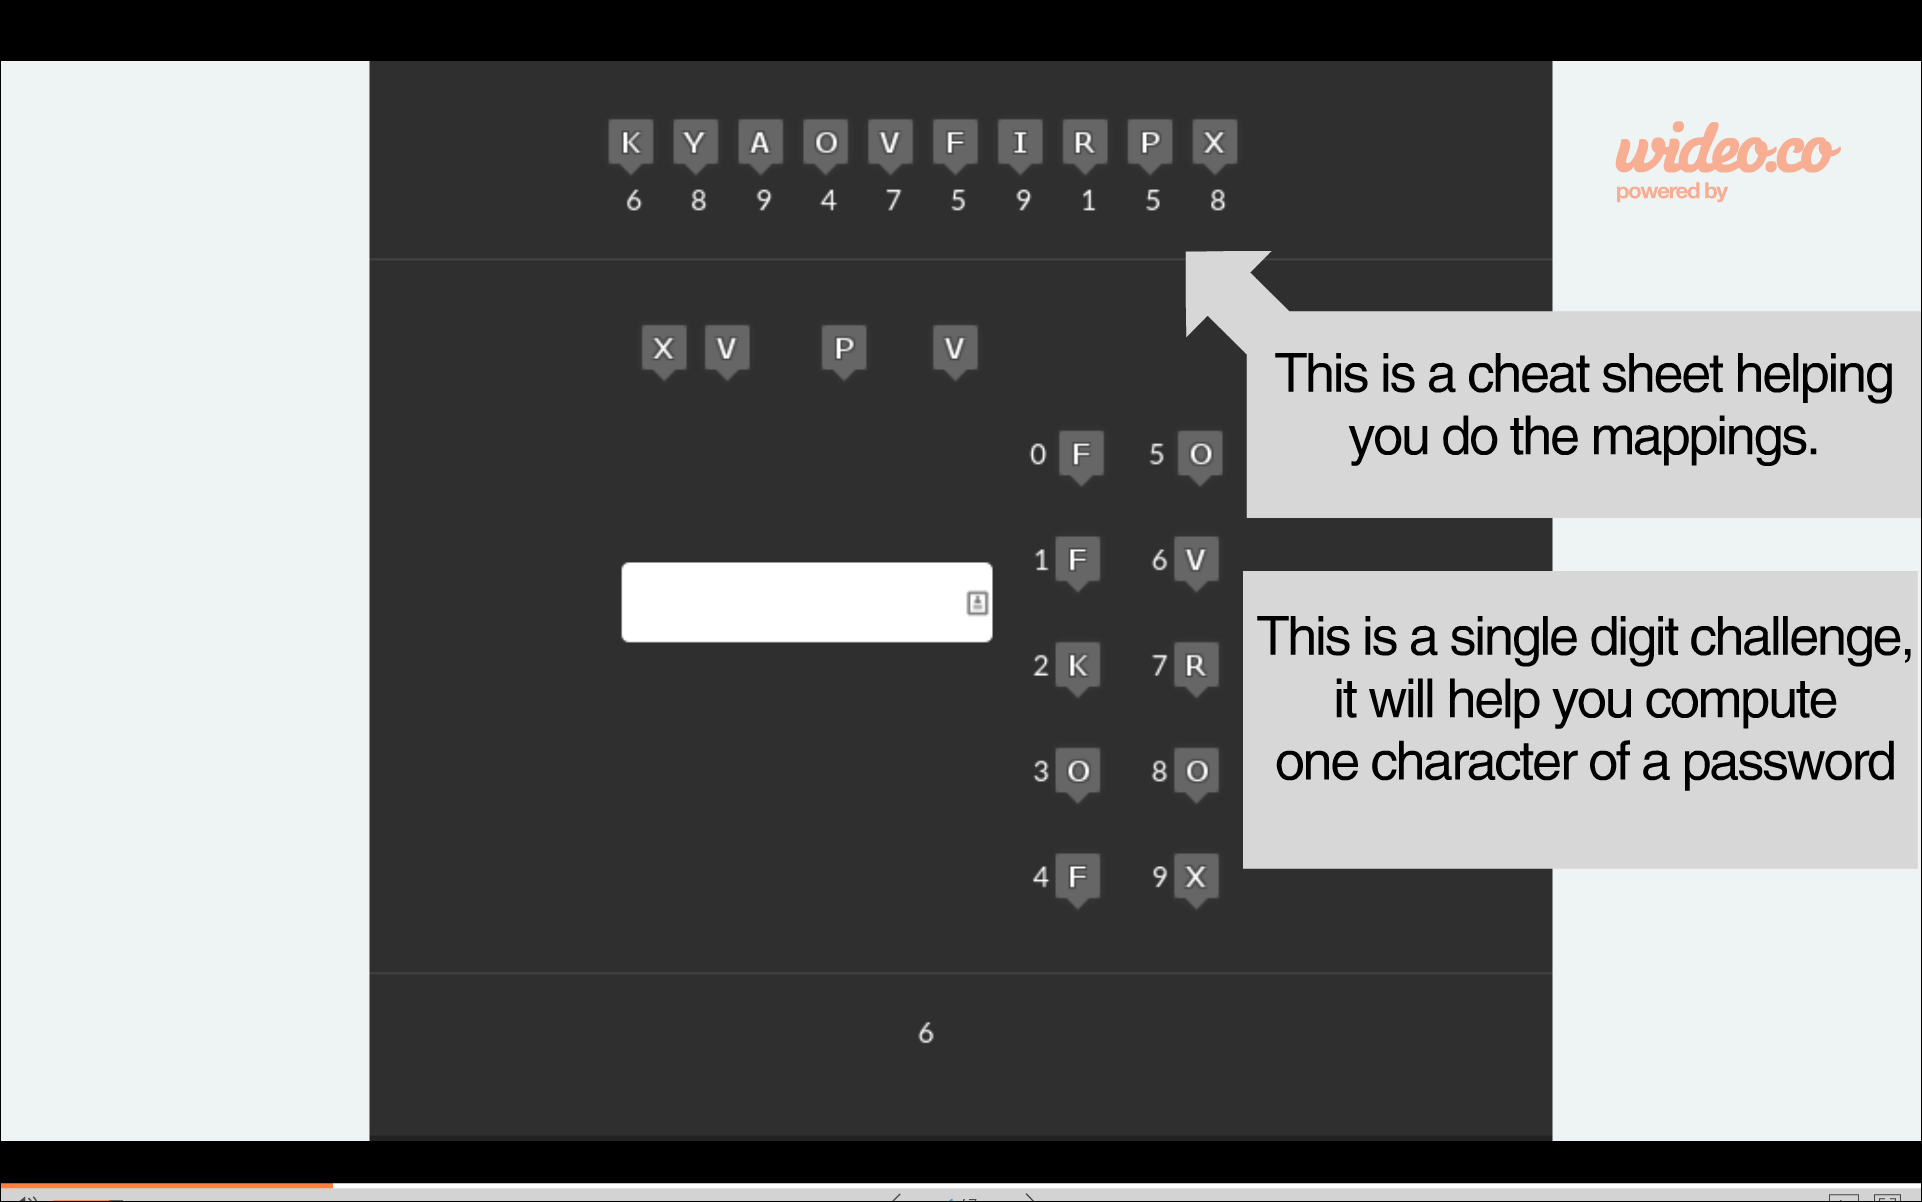
\includegraphics[width=\textwidth]{slides/slide1}
    \caption{Demo slide 1.}
    \label{slide1}
\end{figure}


\begin{figure}
    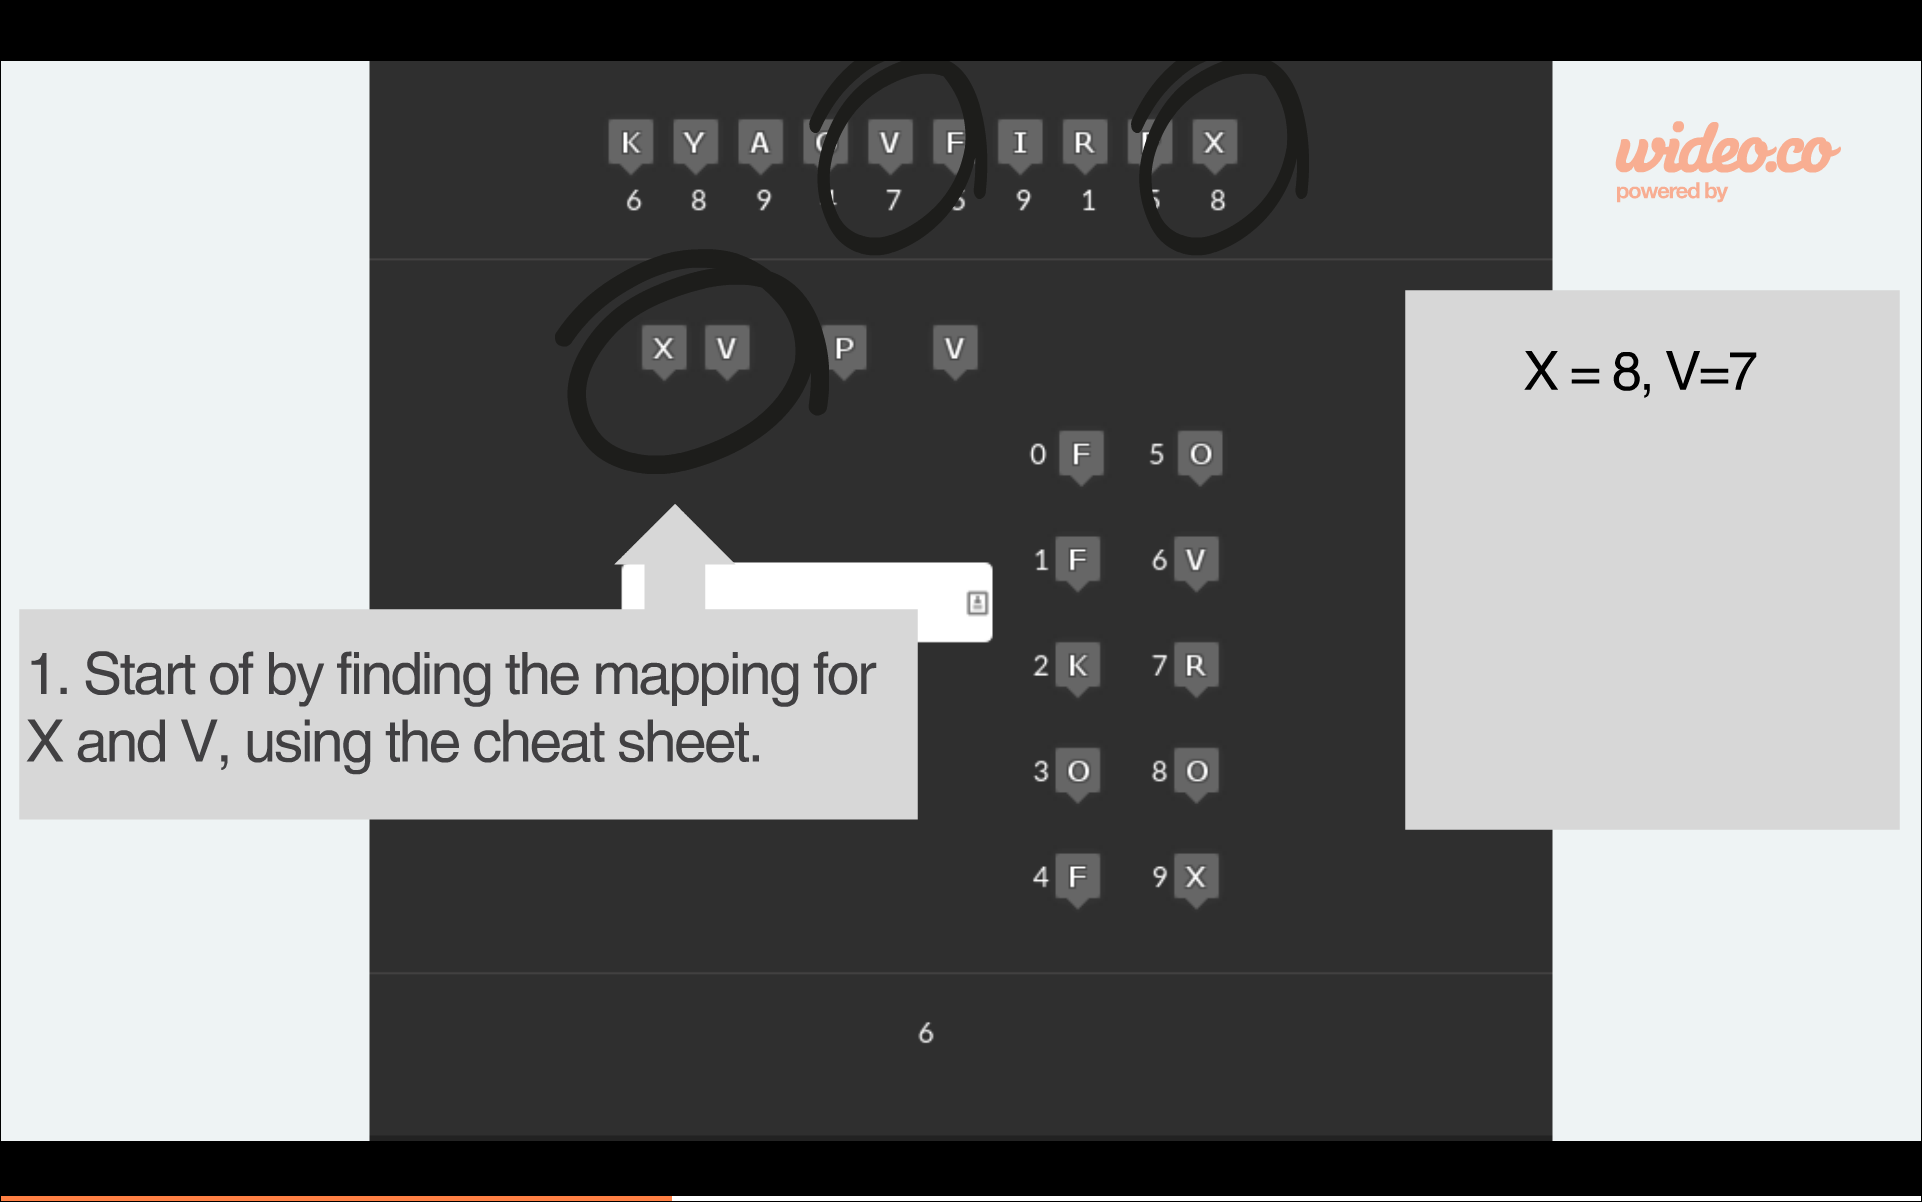
\includegraphics[width=\textwidth]{slides/slide2}
    \caption{Demo slide 2.}
    \label{slide2}
\end{figure}


\begin{figure}
    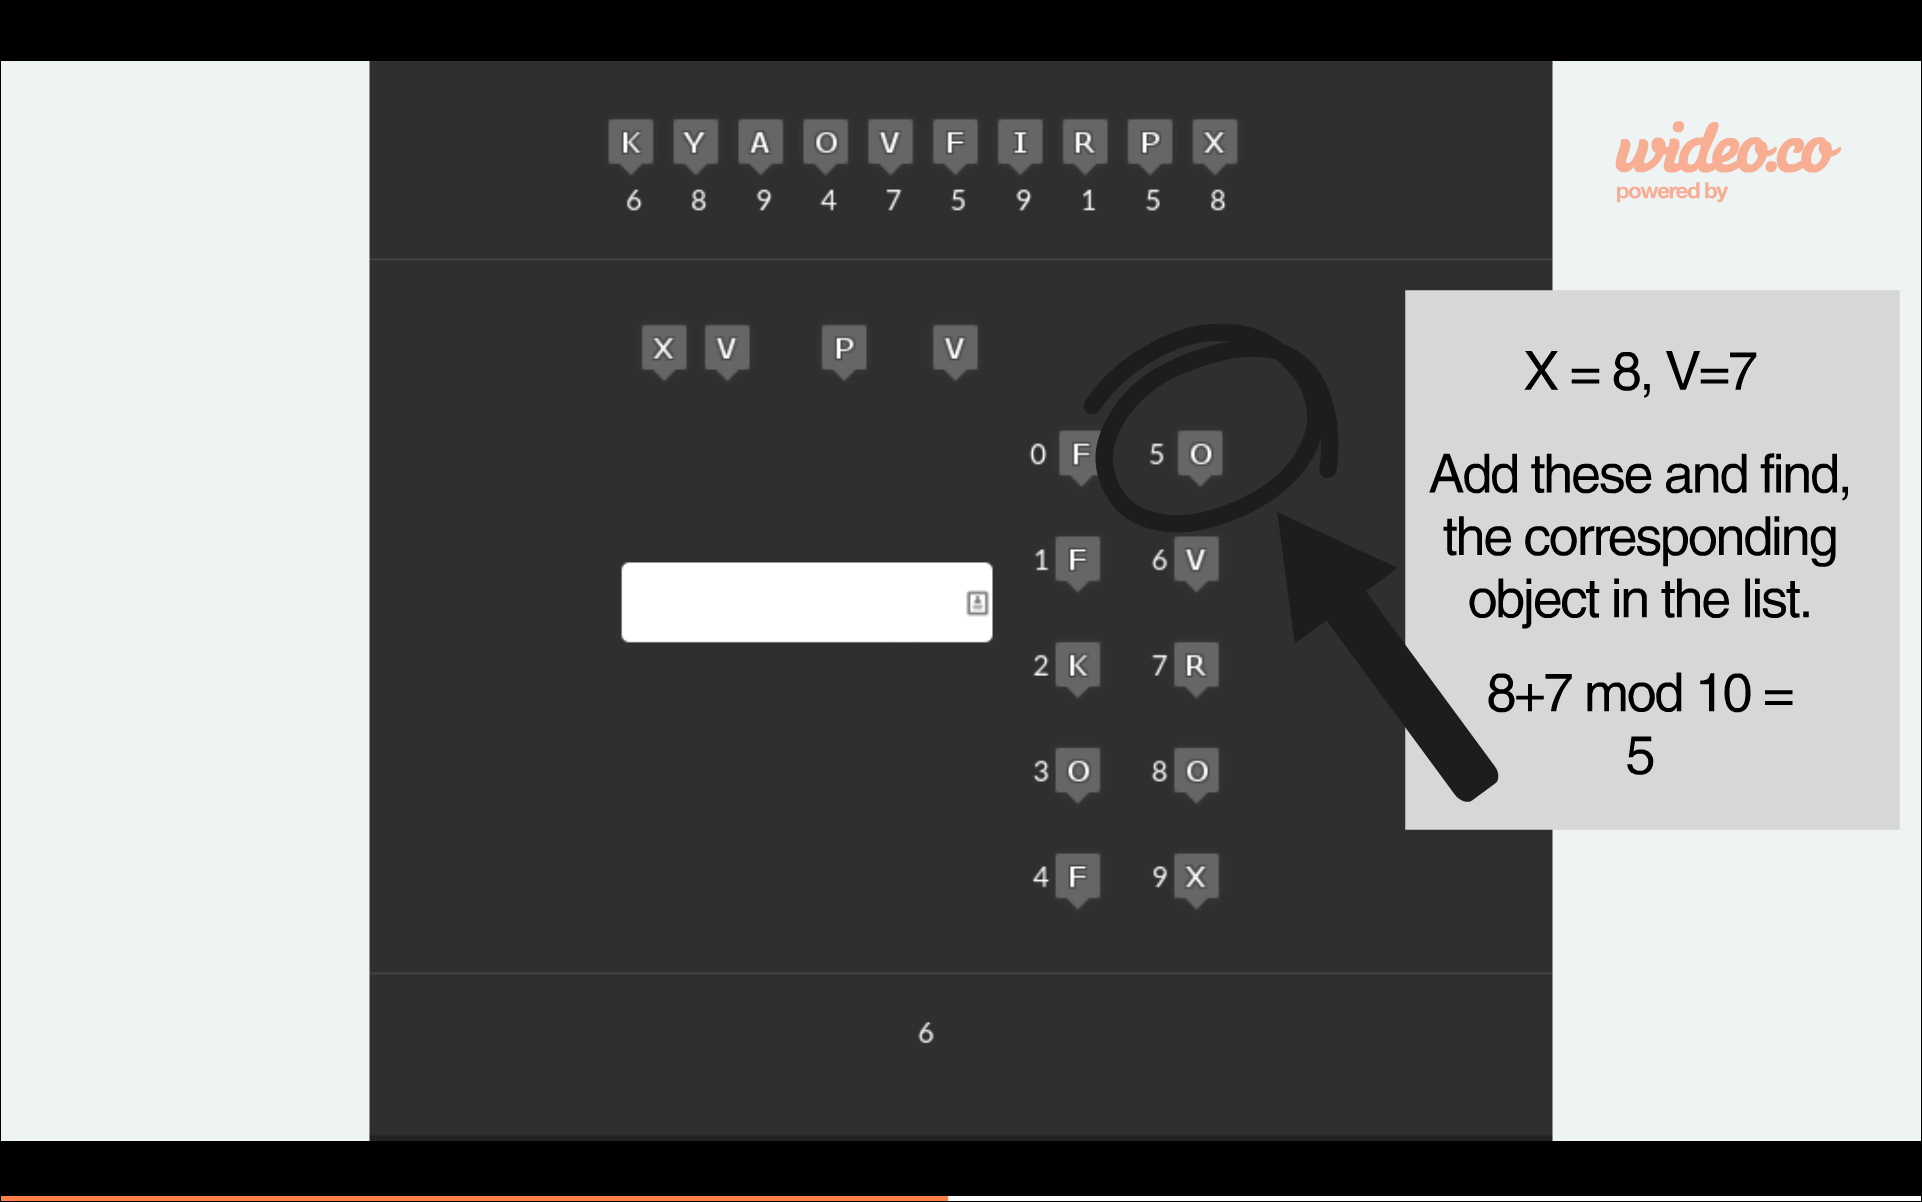
\includegraphics[width=\textwidth]{slides/slide3}
    \caption{Demo slide 3.}
    \label{slide3}
\end{figure}


\begin{figure}
    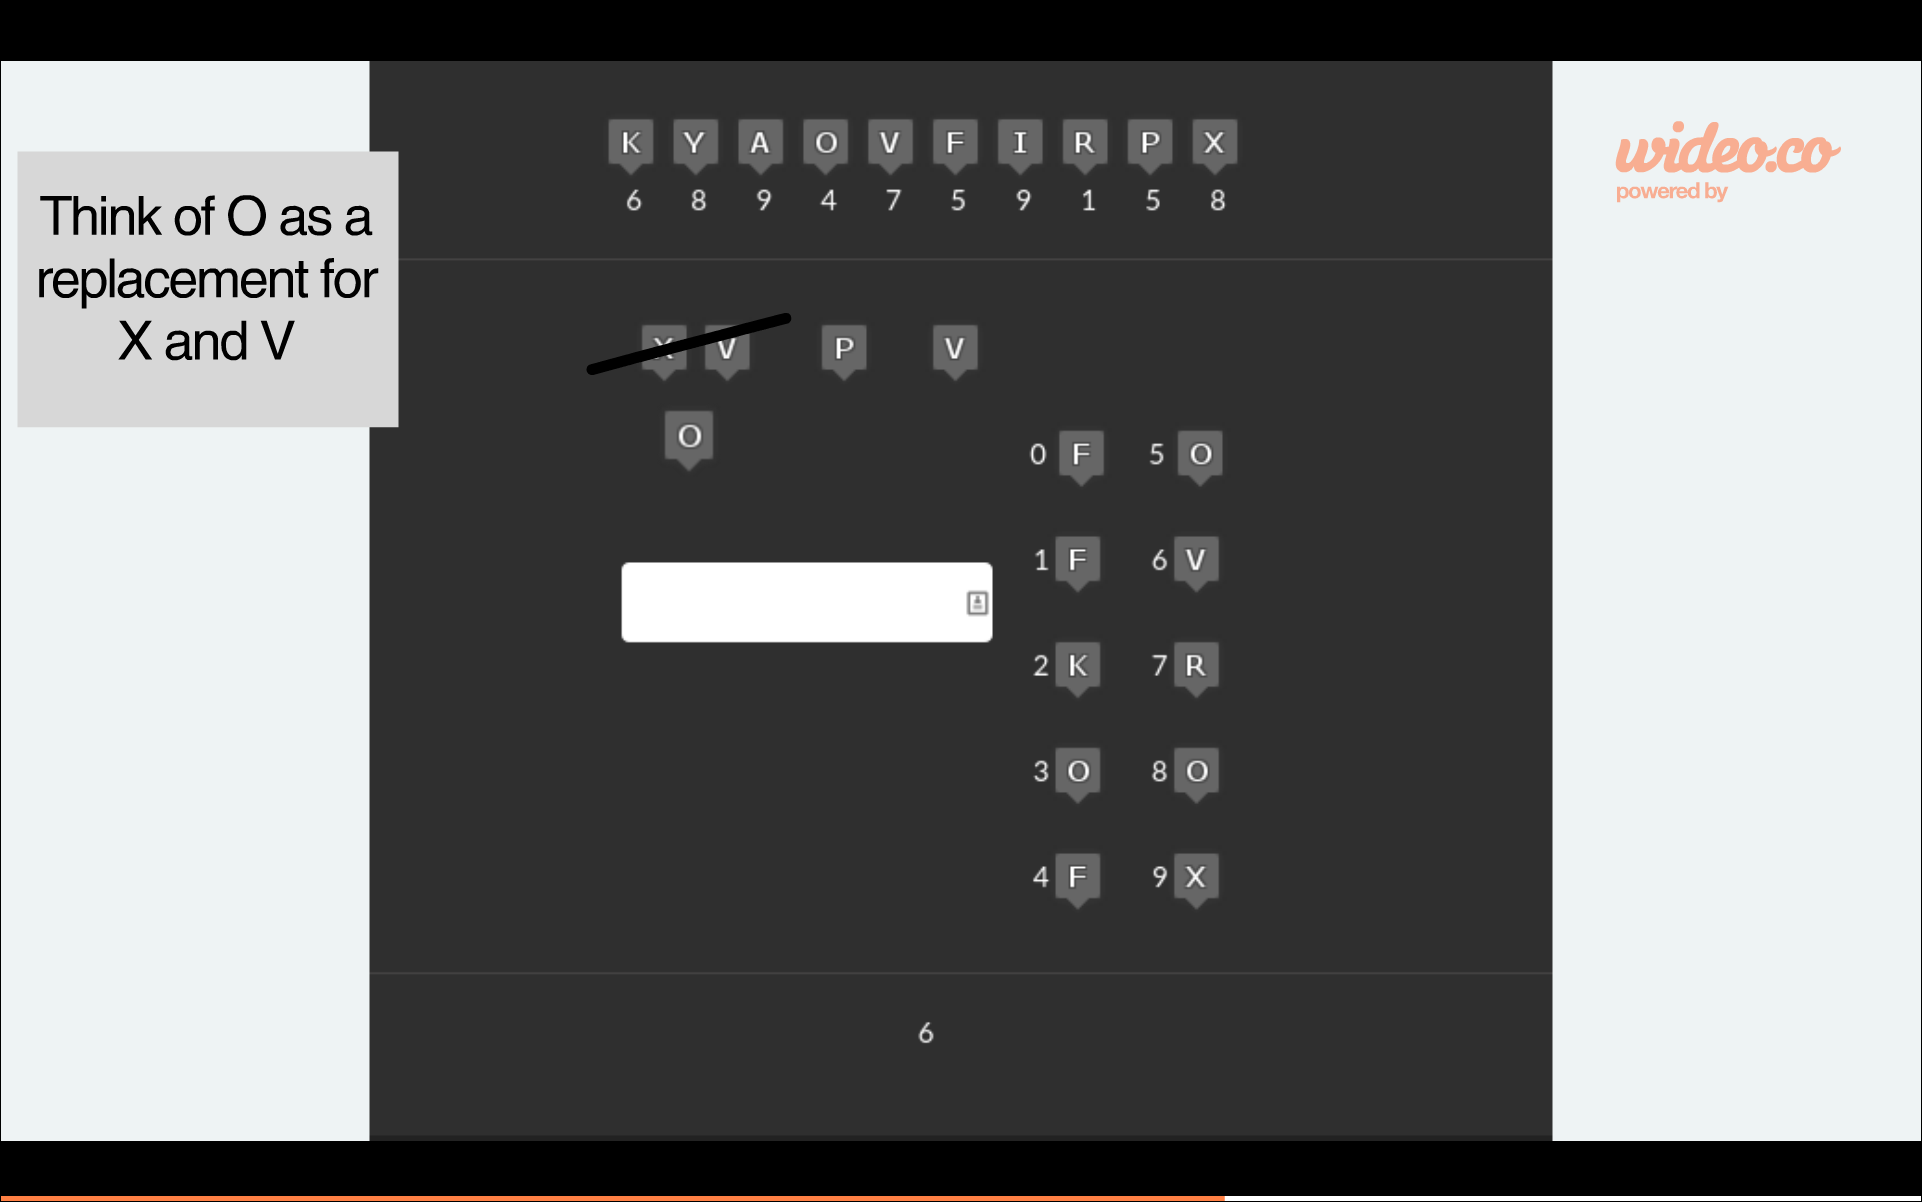
\includegraphics[width=\textwidth]{slides/slide4}
    \caption{Demo slide 4.}
    \label{slide4}
\end{figure}

\begin{figure}
    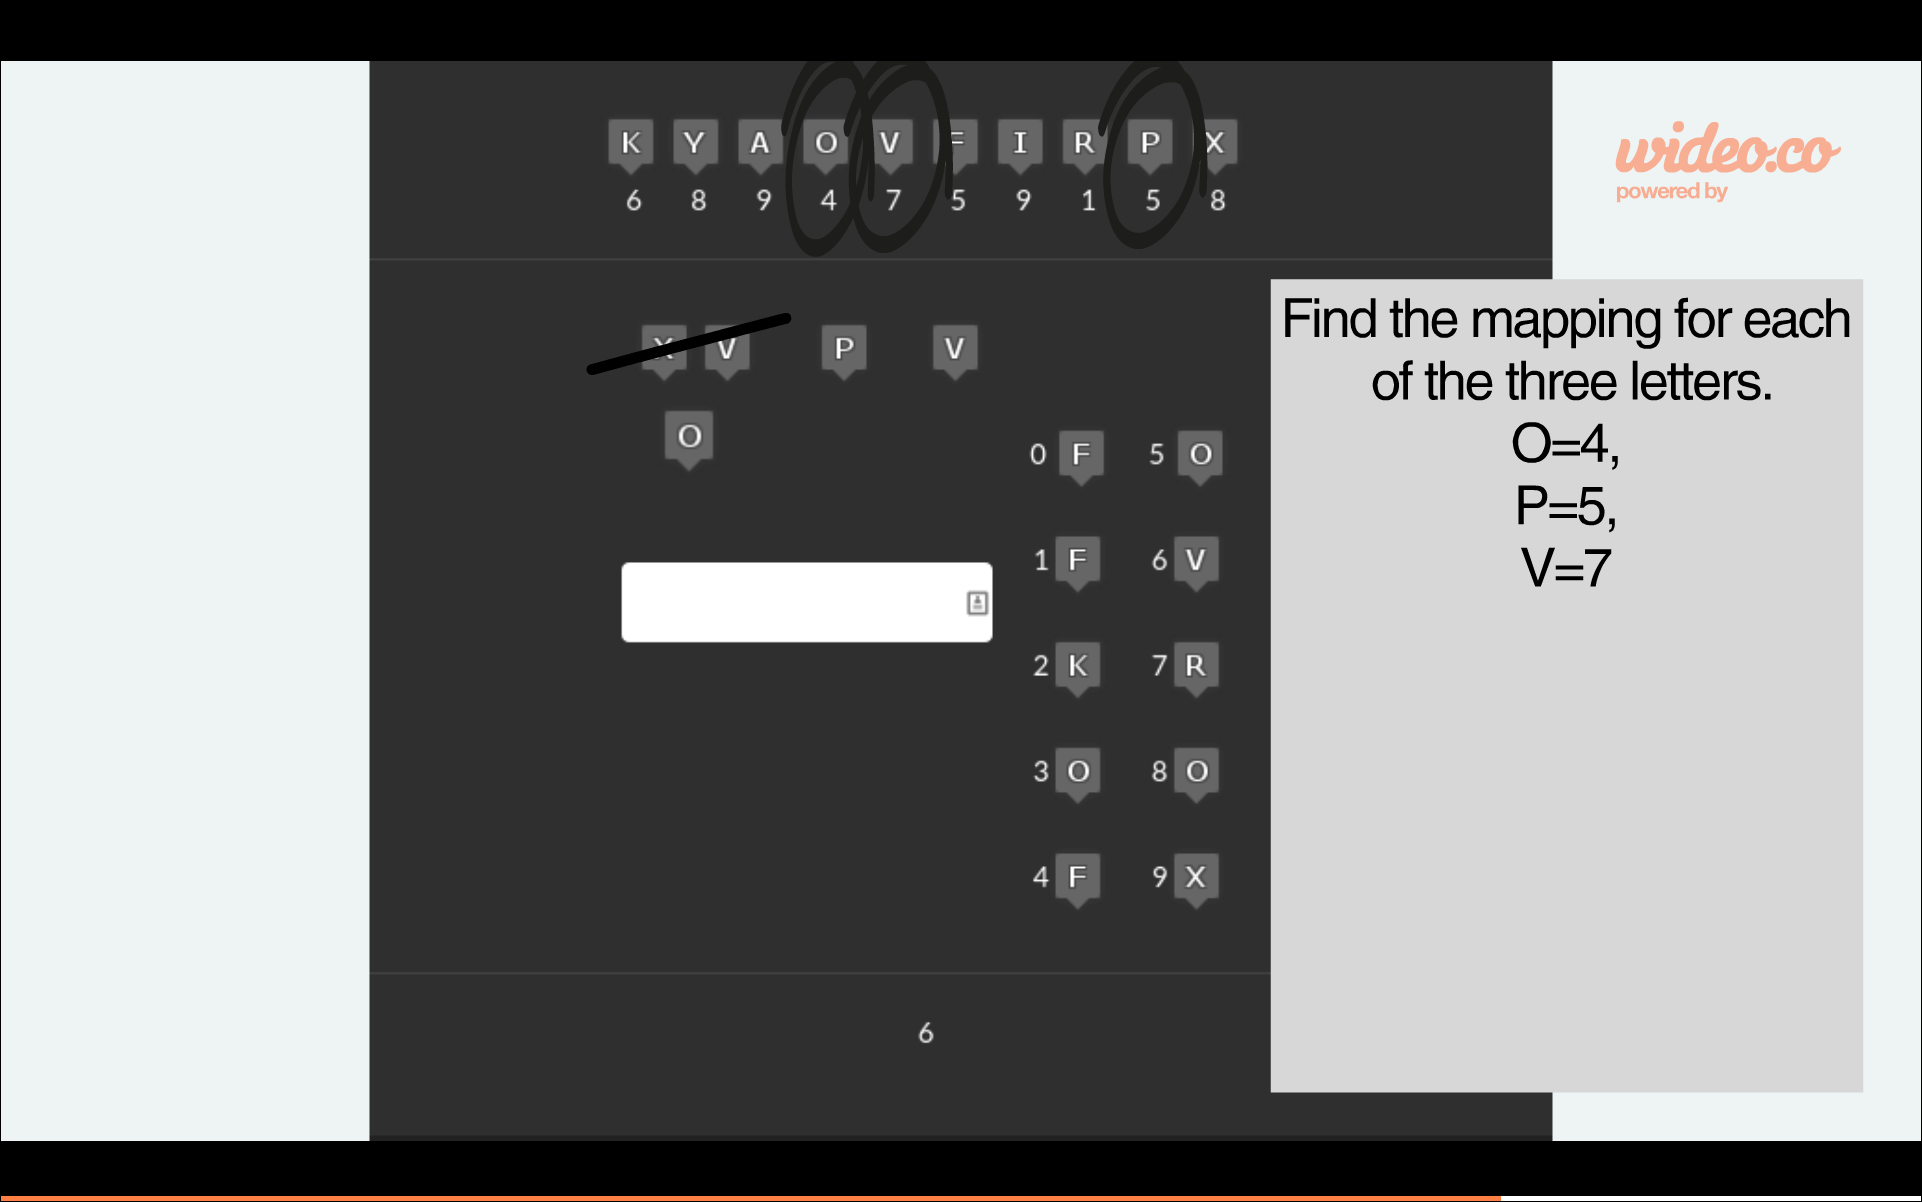
\includegraphics[width=\textwidth]{slides/slide5}
    \caption{Demo slide 5.}
    \label{slide5}
\end{figure}


\begin{figure}
    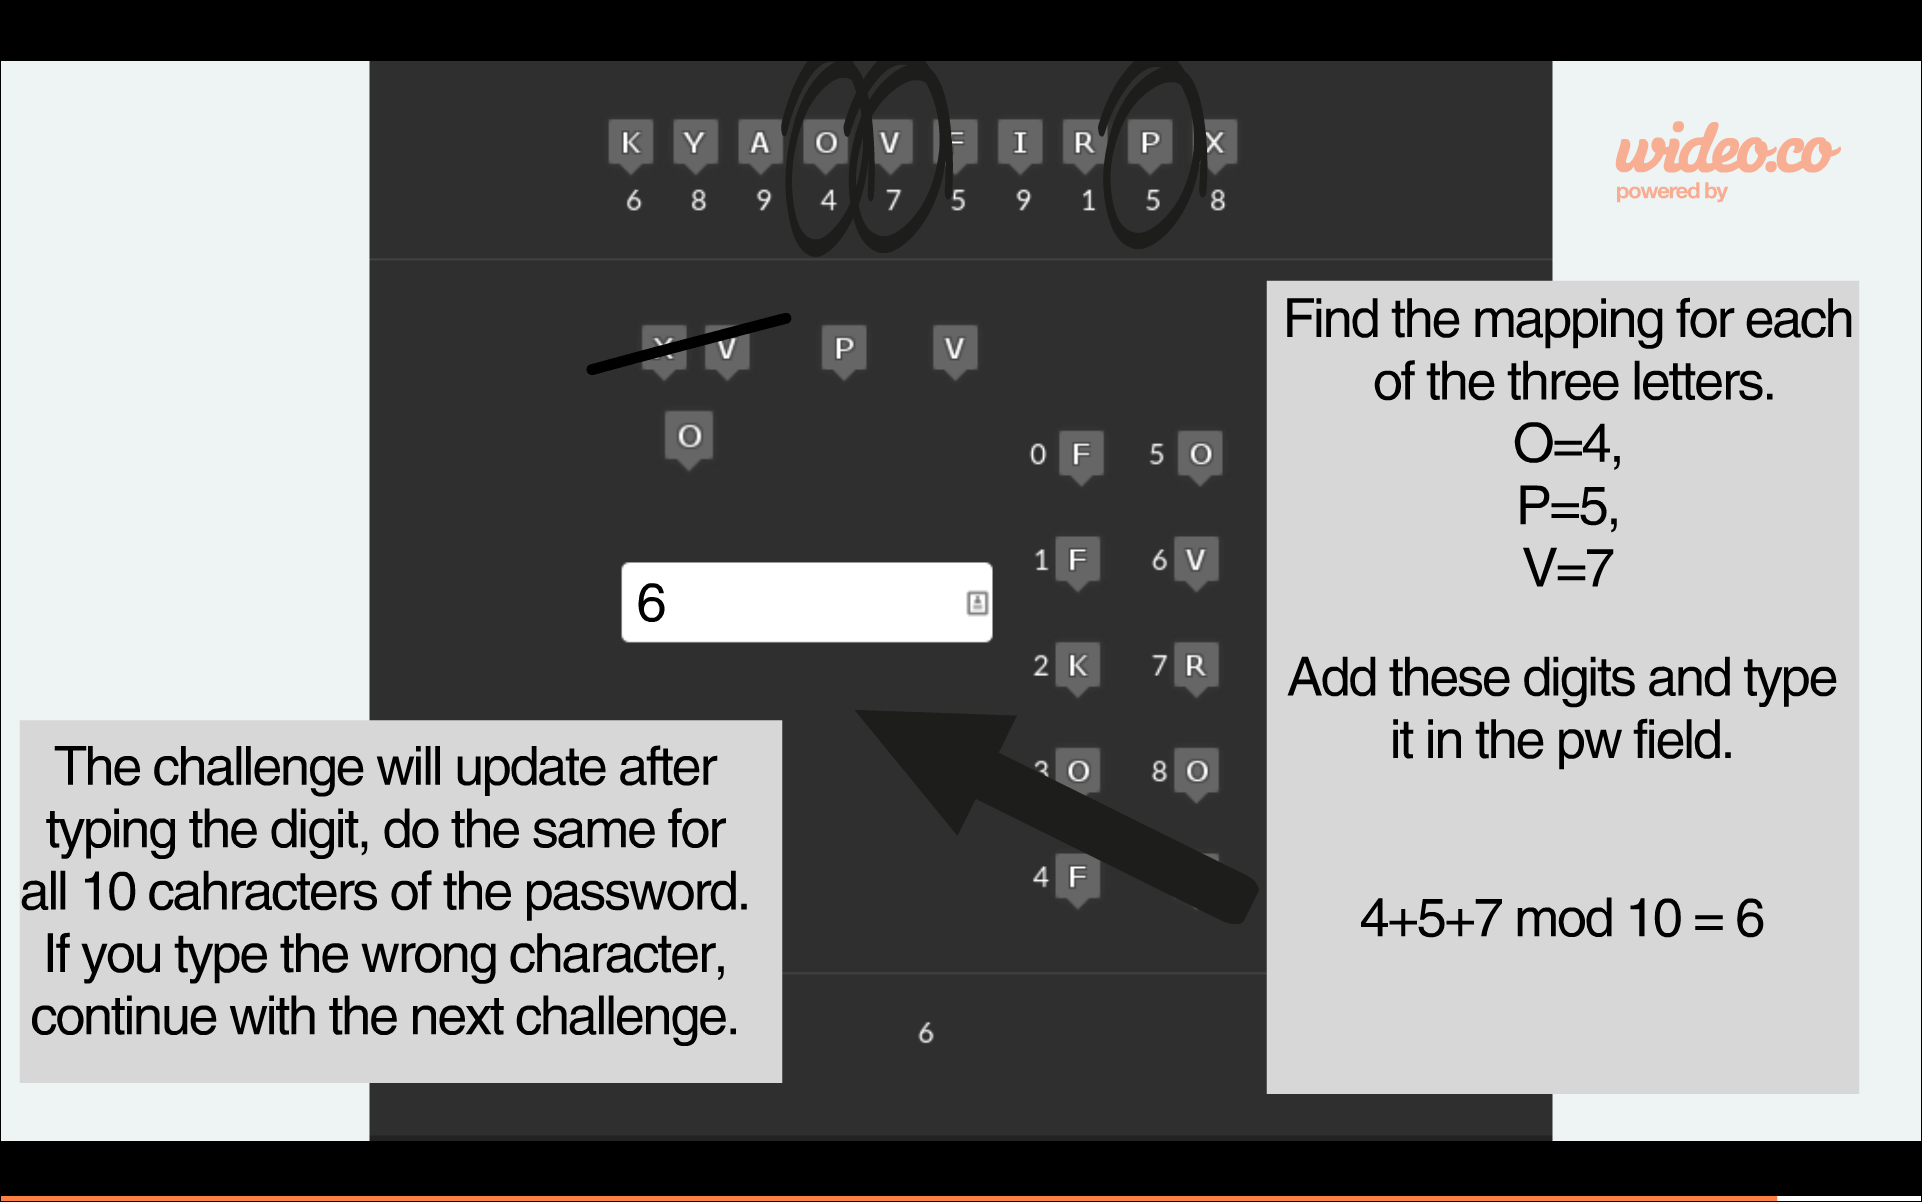
\includegraphics[width=\textwidth]{slides/slide6}
    \caption{Demo slide 6.}
    \label{slide6}
\end{figure}

